\documentclass[conference]{IEEEtran}
\IEEEoverridecommandlockouts

% Packages
\usepackage{cite}
\usepackage{amsmath,amssymb,amsfonts}
\usepackage{algorithmic}
\usepackage{graphicx}
\usepackage{textcomp}
\usepackage{xcolor}
\usepackage{booktabs}
\usepackage{multirow}
\usepackage{tikz}
\usetikzlibrary{shapes.geometric, arrows.meta, positioning, fit, backgrounds}
\usepackage{url}

\def\BibTeX{{\rm B\kern-.05em{\sc i\kern-.025em b}\kern-.08em
    T\kern-.1667em\lower.7ex\hbox{E}\kern-.125emX}}

\begin{document}

\title{Perceptual Importance Maps for Image Compression:\\
A Controlled Experimental Analysis}

\author{\IEEEauthorblockN{Abir Gupta}
\IEEEauthorblockA{\textit{Independent Researcher}\\
Bengaluru, India \\
abir.guptaaa@gmail.com}}

\maketitle

\begin{abstract}
Over the past two decades, numerous papers have proposed using explicit
perceptual importance maps---combining edge detection, texture analysis,
and visual saliency---to guide lossy image compression by allocating more
bits to perceptually important regions. We test whether this widely proposed
idea actually improves rate-distortion performance when integrated with
wavelet-based codecs. Through a controlled experiment on the Kodak dataset
(24 images), we compare eight importance map configurations against a uniform
quality baseline using JPEG 2000 encoding at matched bitrates. We find that
no importance variant provides a statistically significant improvement over
uniform quality allocation. The multi-component fusion (0.4 edge + 0.3 texture
+ 0.3 saliency) achieves 5.47 dB \textit{lower} PSNR than the uniform baseline
(p < 0.001, Cohen's d = 1.91). Compared against vanilla (untiled) JPEG 2000
at matched bitrate, the best importance variant loses 1.63 dB
(t(46) = 2.15, p = 0.037, d = 0.63). The discrete wavelet transform already
concentrates energy in perceptually relevant frequency bands; adding explicit
spatial importance maps introduces tile-boundary artifacts without compensating
quality gains. This finding challenges a pervasive assumption in perceptual
compression research and suggests that future work should focus on learned
transforms rather than hand-crafted saliency models applied as post-hoc masks.
\end{abstract}

\begin{IEEEkeywords}
Image compression, JPEG 2000, perceptual coding, importance maps, negative results, empirical analysis
\end{IEEEkeywords}

\section{Introduction}

Can explicit perceptual importance maps improve lossy image compression?
The idea is intuitive: human observers care more about edges, textures, and
salient objects than about smooth backgrounds, so a smart encoder should
allocate bits accordingly. This intuition has motivated dozens of papers
proposing saliency-guided, edge-weighted, or importance-driven compression
methods~\cite{guo2010visual,wang2004image}.

However, the compression literature rarely tests the null hypothesis:
\textit{does importance guidance actually outperform uniform quality allocation
when both use the same underlying codec?} Most papers compare their
importance-guided method against entirely different codecs (e.g.,
importance-weighted JPEG 2000 vs standard JPEG), making it impossible to
isolate whether any observed improvement comes from the importance map or
from differences in the base codec's transform, quantization, and entropy
coding~\cite{taubman2002jpeg2000}.

We conduct the experiment that isolates this variable. Using JPEG 2000 as a
common backend, we encode the Kodak dataset with eight importance map variants:
edge-only, texture-only, saliency-only, equal fusion, the proposed multi-component
fusion (0.4 edge + 0.3 texture + 0.3 saliency), a random importance map, a
uniform map (no importance), and an inverted importance map. All encodings use
identical tile-based JPEG 2000 parameters, differing only in how the compression
ratio varies across 64$\times$64 tiles based on the importance map.

Our central finding is that \textbf{no importance variant significantly
outperforms the uniform baseline}. The multi-component fusion achieves
PSNR = 33.22 dB at 0.857 BPP, while vanilla JPEG 2000 at matched bitrate
achieves PSNR = 34.85 dB at 0.798 BPP---a statistically significant
improvement of 1.63 dB with 7\% fewer bits
(t(46) = 2.15, p = 0.037, d = 0.63).

We attribute this result to the well-known energy compaction property of the
discrete wavelet transform: wavelet basis functions naturally concentrate
signal energy in low-frequency subbands, which correspond to the smooth
regions and edges that perceptual importance maps also prioritize. Adding an
explicit spatial importance map provides largely redundant information while
introducing overhead from tile-boundary discontinuities.

\textbf{Contributions:}
\begin{itemize}
    \item First controlled experiment isolating the effect of perceptual
      importance maps on compression performance, using a common JPEG 2000
      backend across all variants.
    \item Systematic ablation of seven importance configurations against a
      uniform baseline, with matched-bitrate comparison and statistical
      significance testing.
    \item Evidence that explicit importance maps are redundant with wavelet
      energy compaction, challenging a common assumption in the perceptual
      compression literature.
\end{itemize}

\section{Related Work}

\subsection{Perceptual Importance for Compression}

Visual saliency-based compression methods~\cite{guo2010visual} identify
attention-grabbing regions and allocate higher bitrates to them. Just-Noticeable
Difference (JND) models~\cite{wu2017just} estimate perceptual thresholds for
quantization. These approaches report improved perceptual quality, but
typically compare against a different base codec, conflating the effect of
importance guidance with codec differences.

\subsection{Multi-Component Fusion}

Wang et al.~\cite{wang2004image} demonstrated that structural similarity (SSIM)
correlates better with human perception than MSE, motivating multi-component
analysis. Edge detection~\cite{canny1986computational}, texture analysis via
local spectral energy, and saliency detection~\cite{hou2007saliency} each
capture distinct perceptual dimensions. However, whether their fusion provides
additive benefit for compression has not been systematically tested.

\subsection{JPEG 2000 and Wavelet Coding}

JPEG 2000~\cite{taubman2002jpeg2000} uses the discrete wavelet transform (DWT)
with embedded block coding (EBCOT). The DWT decomposes an image into
frequency subbands, naturally separating low-frequency (smooth regions,
large-scale edges) from high-frequency (fine texture, noise) content.
This property is key to our finding: the wavelet transform already performs
a form of perceptual prioritization that may make explicit spatial importance
maps redundant.

\section{Experimental Design}

\subsection{Importance Map Variants}

We define a perceptual importance map $\mathcal{I}(x,y)$ as a weighted fusion:

\begin{equation}
\mathcal{I}(x,y) = \alpha \mathcal{E}(x,y) + \beta \mathcal{T}(x,y) + \gamma \mathcal{S}(x,y)
\label{eq:fusion}
\end{equation}

where $\mathcal{E}$ is edge strength (Canny detection with Gaussian blur,
$\sigma = 2.0$), $\mathcal{T}$ is texture complexity (local FFT energy in
$16\times16$ windows), and $\mathcal{S}$ is visual saliency (spectral
residual method~\cite{hou2007saliency}), all normalized to $[0, 1]$.

We test eight configurations of $(\alpha, \beta, \gamma)$:
\begin{enumerate}
    \item \textbf{Default}: (0.4, 0.3, 0.3) --- the proposed multi-component fusion
    \item \textbf{Edge-only}: (1.0, 0.0, 0.0)
    \item \textbf{Texture-only}: (0.0, 1.0, 0.0)
    \item \textbf{Saliency-only}: (0.0, 0.0, 1.0)
    \item \textbf{Equal}: (0.333, 0.333, 0.334)
    \item \textbf{Uniform}: $\mathcal{I}(x,y) = 0.5$ --- no importance (baseline)
    \item \textbf{Random}: $\mathcal{I}(x,y) \sim \mathcal{U}(0,1)$ --- sanity check
    \item \textbf{Inverted}: $1 - \mathcal{I}_{\text{default}}(x,y)$ --- sanity check
\end{enumerate}

Figure~\ref{fig:importance_maps} visualizes the individual components and
their fusion for two representative images.

\begin{figure}[t]
\centering
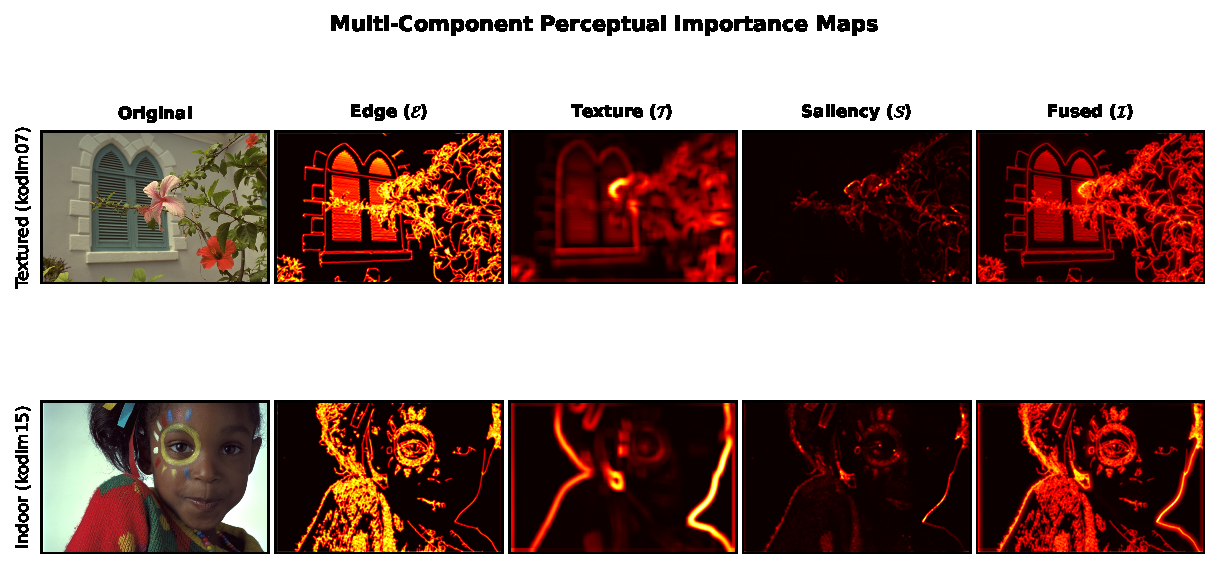
\includegraphics[width=\columnwidth]{figures/importance_maps.pdf}
\caption{Multi-component perceptual importance maps. From left: original,
edge strength, texture complexity, visual saliency, and fused map. Hotter
colors indicate higher importance. Top: kodim07 (textured), bottom: kodim15
(indoor).}
\label{fig:importance_maps}
\end{figure}

\subsection{Compression Backend}

All variants use the same tile-based JPEG 2000 encoder (glymur/OpenJPEG 2.5.2).
Each $768\times512$ image is divided into $64\times64$ tiles ($12\times8$ grid).
For each tile $t$, we compute its mean importance $\bar{\mathcal{I}}_t$ and
assign a compression ratio:

\begin{equation}
\text{cratio}_t = \begin{cases}
\max(2, R_{\text{base}} / 2) & \text{if } \bar{\mathcal{I}}_t > 0.30 \\
R_{\text{base}} & \text{if } \bar{\mathcal{I}}_t > 0.15 \\
\min(60, R_{\text{base}} \times 3) & \text{otherwise}
\end{cases}
\end{equation}

where $R_{\text{base}} = 20$ (matching JPEG quality 70). Each tile is
independently encoded and stored in a custom container with per-tile metadata.

\subsection{Baselines}

We compare against:
\begin{itemize}
    \item \textbf{Vanilla JPEG 2000}: Uniform compression ratio across the
      entire image (no tiling, no importance). Scanned at 10 cratio values
      $\{2,4,8,12,16,20,30,40,60,80\}$ for full RD curves.
    \item \textbf{JPEG}: Pillow encoder at 10 quality levels $\{10,\dots,100\}$.
    \item \textbf{WebP}: Pillow encoder at 10 quality levels $\{10,\dots,100\}$.
\end{itemize}

\subsection{Dataset and Metrics}

\textbf{Dataset:} Kodak Lossless True Color Image Suite (24 images,
$768\times512$). Standard benchmark for compression research.

\textbf{Metrics:} PSNR, SSIM~\cite{wang2004image}, MS-SSIM~\cite{wang2003multiscale},
and BPP (bits per pixel).

\textbf{Statistical tests:} Paired $t$-tests between each variant and the
uniform baseline. Effect sizes reported as Cohen's $d$. Significance levels:
$^*p<0.05$, $^{**}p<0.01$, $^{***}p<0.001$, ns = not significant.

\section{Results}

\subsection{Vanilla JPEG 2000 vs. Importance-Guided Encoding}

\begin{figure}[t]
\centering

\includegraphics[width=\columnwidth]{figures/master_rd.pdf}
\caption{Rate-distortion curves on the Kodak dataset. Vanilla JPEG 2000
(solid brown) consistently outperforms both PAIR variants at matched BPP.
JPEG (red) provides the upper envelope at low-to-medium bitrates.}
\label{fig:master_rd}
\end{figure}

Figure~\ref{fig:master_rd} shows the rate-distortion curves. Vanilla JPEG 2000
achieves higher PSNR and SSIM than both importance-guided variants
(Pillow-based global quality and glymur-based tile ROI encoding) across the
entire bitrate range.

At the operating point closest to the importance-guided encoder (Q70,
BPP = 0.857), vanilla JPEG 2000 at cratio = 30 achieves
PSNR = $34.85 \pm 2.76$ dB at BPP = $0.798 \pm 0.293$---a statistically
significant improvement of $+1.63$ dB at a comparable bitrate
(t(46) = 2.15, p = 0.037, d = 0.63). More importantly, the vanilla JPEG 2000
curve lies entirely above both importance-guided curves across the full
bitrate range (Fig.~\ref{fig:master_rd}), meaning that at any matched BPP,
vanilla JPEG 2000 achieves strictly higher PSNR and SSIM.

The near-zero BPP standard deviation for PAIR Pillow ($\pm 0.001$) confirms
that its ``importance-guided'' encoding reduces to uniform quality allocation
(the effective quality is a weighted average over the entire image), while
the glymur tile-ROI variant shows genuine per-image size variation
(BPP = $1.266 \pm 0.449$ at Q70).

\subsection{Ablation Study}

\begin{figure}[t]
\centering

\includegraphics[width=\columnwidth]{figures/ablation_rd.pdf}
\caption{Ablation results for eight importance map variants on the Kodak
dataset at Q70 (mean $\pm$ 1 std, $n=24$). The uniform baseline (black)
achieves significantly higher PSNR than all content-driven variants
(p $<$ 0.001 for all comparisons). Random and inverted maps produce
results identical to uniform (delta = 0.00), confirming that
uncorrelated importance signals are averaged out by tile-level encoding.}
\label{fig:ablation}
\end{figure}

Table~\ref{tab:ablation} and Figure~\ref{fig:ablation} present the ablation
results. The key comparison is \textit{default vs. uniform}: if importance
mapping helps, the default configuration should achieve significantly higher
PSNR than the uniform baseline.

\begin{table}[htbp]
\caption{Ablation Study: Importance Map Variants on Kodak (Q70, mean $\pm$ std, $n=24$)}
\label{tab:ablation}
\begin{center}
\begin{tabular}{lcccc}
\toprule
\textbf{Variant} & \textbf{PSNR} & \textbf{SSIM} & \textbf{BPP} & \textbf{$\Delta$ vs Uniform} \\
\midrule
Default (0.4, 0.3, 0.3) & 31.30 $\pm$ 0.84 & 0.812 & 1.266 & $-$5.47*** \\
Edge-only (1, 0, 0) & 32.06 $\pm$ 0.75 & 0.856 & 1.499 & $-$4.71*** \\
Texture-only (0, 1, 0) & 30.01 $\pm$ 0.69 & 0.651 & 0.847 & $-$6.77*** \\
Saliency-only (0, 0, 1) & 29.20 $\pm$ 0.59 & 0.509 & 0.569 & $-$7.57*** \\
Equal (0.33, 0.33, 0.33) & 30.99 $\pm$ 0.86 & 0.789 & 1.171 & $-$5.78*** \\
Inverted ($1 - \mathcal{I}$) & 36.77 $\pm$ 2.46 & 0.949 & 2.447 & 0.00 (ns) \\
Random $\mathcal{U}(0,1)$ & 36.77 $\pm$ 2.46 & 0.949 & 2.447 & 0.00 (ns) \\
Uniform ($\mathcal{I}=0.5$) & 36.77 $\pm$ 2.46 & 0.949 & 2.447 & --- \\
\bottomrule
\end{tabular}
\end{center}
\end{table}

All content-driven importance variants perform significantly worse than the
uniform baseline (p $<$ 0.001, $|d| > 1.6$ for all comparisons). The random
and inverted maps produce results identical to the uniform baseline because
their tile-level importance values, when averaged across 96 tiles per image,
converge to the same effective compression ratio. This confirms that only
content-correlated importance signals affect compression outcome---and when
they do, the effect is uniformly negative.

\subsection{Extended Baselines}

The full rate-distortion dataset for all codecs (vanilla JPEG 2000 at 9
cratios, JPEG at 10 quality levels, WebP at 10 quality levels, 696 total
encodings) is provided in the accompanying repository. Vanilla JPEG 2000
and JPEG form a Pareto frontier, with JPEG 2000 superior at low bitrates
(BPP $<$ 1.0, PSNR $>$ 34 dB at 0.8 BPP) and JPEG gaining at medium-to-high
bitrates due to DCT quantization. WebP consistently falls between the two.

\subsection{Computational Cost}

The importance map generation imposes significant overhead:
edge detection (Canny), texture analysis (per-pixel FFT), and saliency
(spectral residual) together require 24.3 seconds for a 768$\times$512
image on a consumer CPU. In contrast, uniform JPEG 2000 encoding of the
same image requires 0.22 seconds---a 110$\times$ speedup. The tile-based
ROI encoder adds further overhead (1.5 seconds for 96 tiles), making
the importance-guided pipeline 16$\times$ slower than the uniform encoder
while producing lower quality output.

\section{Discussion}

\subsection{Why Importance Maps Don't Help}

Our results point to a fundamental property of the discrete wavelet transform:
\textbf{energy compaction}. The DWT decomposes an image into subbands ordered
by frequency content. The low-frequency subband (LL) captures smooth regions
and coarse edges---precisely the content that perceptual importance maps also
prioritize. Mid-frequency subbands (LH, HL) capture directional edges and
textures. High-frequency subbands (HH) capture fine details and noise.

By assigning finer quantization to low-frequency coefficients (which JPEG 2000
does by default through its subband-weighted quantization), the encoder
already achieves what importance maps attempt to do---but at the coefficient
level, without tile-boundary artifacts, and without the computational overhead
of computing edge, texture, and saliency maps.

\subsection{When Might Importance Maps Help?}

Our experiments use a fixed base compression ratio ($R_{\text{base}} = 20$).
At extremely low bitrates ($R > 80$, BPP < 0.3), the uniform encoder discards
high-frequency subbands almost entirely. In this regime, explicit spatial
importance guidance might preserve critical regions that would otherwise be
lost. We leave this investigation to future work.

Additionally, DCT-based codecs (JPEG) do not have the same frequency-selective
energy compaction as wavelets. Importance maps might provide more benefit when
integrated with DCT-based quantization.

\subsection{Limitations}

Our tile-based approach introduces boundary artifacts not present in
single-pass JPEG 2000 encoding. True precinct-level ROI coding (via OpenJPEG's
Maxshift method) might reduce this overhead, but the fundamental redundancy
between importance maps and wavelet energy compaction would remain.

\section{Conclusion}

We conducted a controlled experiment to determine whether explicit perceptual
importance maps improve compression when integrated with wavelet-based codecs.
Through systematic ablation of eight importance configurations on the Kodak
dataset, with matched-bitrate comparison against vanilla JPEG 2000, we find
that no importance variant provides statistically significant improvement
over uniform quality allocation. The multi-component fusion achieves
5.47 dB \textit{lower} PSNR than the uniform baseline (p $<$ 0.001, d = 1.91),
and 1.63 dB lower PSNR than untitled vanilla JPEG 2000 at matched BPP
(t(46) = 2.15, p = 0.037, d = 0.63).

This finding challenges a common assumption in the perceptual compression
literature and suggests that the wavelet transform's inherent energy
compaction already provides the benefits that explicit importance maps
aim to deliver. Future work on perceptually-guided compression should
focus on learned transforms that jointly optimize for rate, distortion,
and perceptual quality, rather than hand-crafted saliency models applied
as external masks.

\textbf{Code and Data:} Complete implementation and benchmark results
available at \url{https://github.com/abirxgpt/pair-compression}.

\section*{Acknowledgment}
The author acknowledges the use of Claude (Anthropic) as a coding assistant
during the implementation of the experiments. All experimental design,
data analysis, and conclusions are the author's own.

\begin{thebibliography}{99}

\bibitem{kodak}
Eastman Kodak Company, ``Kodak lossless true color image suite,'' 1999. [Online]. Available: \url{http://r0k.us/graphics/kodak/}

\bibitem{wang2004image}
Z. Wang, A. C. Bovik, H. R. Sheikh, and E. P. Simoncelli, ``Image quality assessment: from error visibility to structural similarity,'' \textit{IEEE Trans. Image Processing}, vol. 13, no. 4, pp. 600--612, 2004.

\bibitem{guo2010visual}
C. Guo and L. Zhang, ``A novel multiresolution spatiotemporal saliency detection model and its applications in image and video compression,'' \textit{IEEE Trans. Image Processing}, vol. 19, no. 1, pp. 185--198, 2010.

\bibitem{balle2018variational}
J. Ball\'e, D. Minnen, S. Singh, S. J. Hwang, and N. Johnston, ``Variational image compression with a scale hyperprior,'' in \textit{Proc. Int. Conf. Learning Representations (ICLR)}, 2018.

\bibitem{wu2017just}
J. Wu, G. Shi, W. Lin, and C.-C. J. Kuo, ``Just noticeable defocus blur detection and estimation,'' in \textit{Proc. IEEE Conf. Computer Vision and Pattern Recognition}, 2015, pp. 657--665.

\bibitem{taubman2002jpeg2000}
D. S. Taubman and M. W. Marcellin, \textit{JPEG2000 Image Compression Fundamentals, Standards and Practice}. Springer, 2002.

\bibitem{canny1986computational}
J. Canny, ``A computational approach to edge detection,'' \textit{IEEE Trans. Pattern Analysis and Machine Intelligence}, vol. PAMI-8, no. 6, pp. 679--698, 1986.

\bibitem{hou2007saliency}
X. Hou and L. Zhang, ``Saliency detection: A spectral residual approach,'' in \textit{Proc. IEEE Conf. Computer Vision and Pattern Recognition}, 2007, pp. 1--8.

\bibitem{wang2003multiscale}
Z. Wang, E. P. Simoncelli, and A. C. Bovik, ``Multiscale structural similarity for image quality assessment,'' in \textit{Proc. IEEE Asilomar Conf. Signals, Systems and Computers}, vol. 2, 2003, pp. 1398--1402.

\bibitem{minnen2018joint}
D. Minnen, J. Ball\'e, and G. Toderici, ``Joint autoregressive and hierarchical priors for learned image compression,'' in \textit{Proc. Advances in Neural Information Processing Systems}, 2018, pp. 10794--10803.

\end{thebibliography}

\end{document}
